\chapter{Implementación de datos estructurados}
\label{chap:4}
En este capítulo, finalmente, nos toca hablar del primero de los dos sistemas implementados en este trabajo.
El sistema en cuestión implementa, con algunas limitaciones que mencionaremos, el modelo de Popescu descripto en \cite{QADB1} y \cite{QADB2} y reseñados por nosotros en \ref{subsec:closed-domain}.


Cabe notar que, al igual que muchos otros trabajos de área, los que utilizamos describen, con mayor o menor detalle, una implementación del modelo teórico, pero el código en sí mismo no es accesible. Nuestro código, por su parte, está accesible públicamente en la siguiente dirección: github. Allí pueden encontrarse, además del código en sí mismo, los procedimientos de instalación, ejemplos de ejecución y una lista con los principales puntos técnicos que pueden mejorarse (ver, también, \allref{subsec:popescu-cierre}).


Testeamos este sistema sobre la base de datos World, en inglés, ofrecida por MySQL\footnote{Ver \url{http://dev.mysql.com/doc/world-setup/en/index.html} y \url{http://dev.mysql.com/doc/index-other.html}} que consta de información geográfica básica sobre países, ciudades e idiomas.

Cabe mencionar que el scope original de este sistema era ser bilingüe y ejecutarse sobre una base de datos sobre universidades, empresas e investigación nacional del ámbito de la informática. Lamentablemente, por una cuestión de tiempos y de errores a la hora de estimar esfuerzos, no pudimos completar este plan original. En la sección \allref{subsec:popescu-cierre} presentamos un roadmap para estas adaptaciones.

La estructura del capítulo es como sigue: En \ref{sec:popescu-db} pasamos revista de la base de datos que utilizamos para testear el sistema y en \ref{sec:popescu-implementacion} discutimos la implementación. \ref{subsec:popescu-codigo} se divide, a su vez, en \ref{subsec:popescu-ejemplos}, donde discutimos la implementación en sí misma, 4.2.2, donde mostramos y comentamos algunos ejemplos de ejecuciones y \ref{subsec:popescu-cierre} donde analizamos los alcances, los límites y el trabajo futuro.


\section{Base de datos}
\label{sec:popescu-db}

La base de datos World consta de 3 tablas: Country, City y CountryLanguage (ver Figura \ref{fig:world-db}).

\begin{figure}
  \centering
    %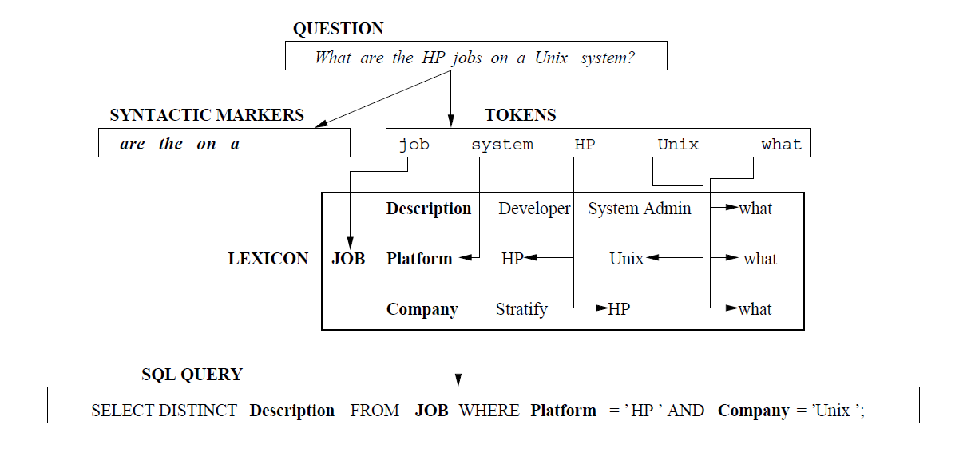
\includegraphics[scale=1.0]{graficos/popescu-example}
    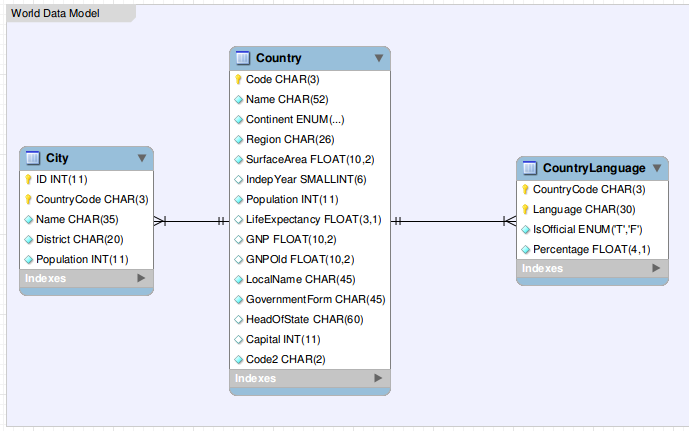
\includegraphics[width=12.823cm,height=8.004cm]{graficos/fuentes/world-db.png}
  \caption{Modelo entidad relación de la base de datos World original}
  \label{fig:world-db}
\end{figure}

La tabla Country tiene información básica acerca de varios países del mundo. La tabla City tiene información sobre las mayores ciudades del mundo y, finalmente, la tabla CountryLanguage tiene información sobre los idiomas hablados en cada país.

Hay una relación de uno a muchos entre Country y CountryLanguage: cada país puede tener más de un idioma y, además, hay una relación de uno a muchos entre Country y City: cada país puede tener más de una ciudad.

\medskip
Las definiciones de las relaciones originales son:
\begin{itemize}
\item Country(Code, Name, Continent, Region, SurfaceArea, IndepYear, Population, LifeExpectancy, GNP, GNPOld, LocalName, GovernmentForm, HeadOfState, Capital, Code2)
\item City(ID, ContryCode, Name, District, Population)
\item CountryLanguage(CountryCode, Language, IsOfficial, Percentage)
\end{itemize}


Para nuestro proyecto, renombramos algunos de los elementos:
\begin{itemize}
\item La relación CountryLanguage fue renombrada a Language
\item El atributo Language de la relación CountryLanguage fue renombrado a Name
\item El atributo IndepYear de la relación Country fue renombrado a IndependenceYear
\end{itemize}

En las tablas X, Y, Z pueden verse algunas filas de ejemplo de cada una de las tablas y, en la tabla W, el total de filas de cada una.
%TODO: HACER TABLAS!!!

Incorporando estos datos al modelo teórico, hasta aquí tenemos definidos: la base de datos, sus elementos ($E$) y el tipo de sus elementos.


\section{Implementación}
\label{sec:popescu-implementacion}

El código de la implementación está disponible en github: acá. Está implementado en java e implementa, con la mayor fidelidad posible, el sistema propuesto por Popescu y descripto en \allref{subsec:closed-domain}.
%TODO: acá

Estructuramos esta sección como sigue. Primero (\ref{subsec:popescu-codigo}), discutimos la implementación en sí misma, analizando los módulos más importantes del sistema  (\ref{subsubsec:lexicon}, etc), luego (\ref{subsec:popescu-ejemplos}) mostramos y comentamos algunos ejemplos de ejecuciones y, finalmente ((\ref{subsec:popescu-cierre})), analizamos analizamos alcances, límites y trabajo futuro.
%TODO: completar las referencias a subsubsections

\subsection{Código}
\label{subsec:popescu-codigo}

Estructura general y librerías usadas y principales módulos
Lexicon: (wordnet + edu.mit.jwi)
%TODO: Hace intro de código

\subsubsection*{Lexicón}
\label{subsubsec:lexicon}
El lexicón, recordemos, es el módulo encargado de generar un conjunto de tokens para cada  elemento de la base de datos. Una vez construido este conjunto, las responsabilidades del módulo son las siguientes:
\begin{itemize}
	\item Dado un lema, devolver el conjunto de tokens que lo contienen
	\item Dado un token, devolver el conjunto de elementos de la base de datos que le \textit{corresponden}.
\end{itemize}

El lexicón está implementado en la clase $uba.modules.Lexicon$. Debemos distinguir los momentos de construcción y de consulta del mismo. La construcción, cuyo punto de entrada es el módulo $uba.app.CreateLexicon$, ocurre por separado, y debe ejecutarse una vez antes de poder utilizar el sistema para responder preguntas. Esta genera 4 archivos con formato json, que son luego cargados en memoria al momento de realizar consultas.

En el centro la construcción del lexicón se encuentra Wordnet (una base de datos léxica en inglés, que consta de conjuntos de sinónimos, definiciones de los mismos y relaciones semánticas entre ellos). Utilizamos esta base de datos para obtener los sinónimos de los elementos de la base de datos.

El input del algoritmo es la lista de los elementos de la base de datos (relaciones, atributos y valores) como strings. El primer paso es eliminar el camel case y separar y lematizar las palabras (la tokenizamos en el sentido dado por Popescu a token). Por ejemplo, después de este paso, el elemento GovernmentForm se convierte en el token \{government, form\}. En este paso eliminamos también las stopwords (por ejemplo, HeadOfState se convierte en \{head, state\}).

Luego, los datos paran por el TokenAugmenter, que simplemente agrega algunos sinónimos escritos a mano a algunos de estos elementos. Por ejemplo, para el elemento region (atributo de la relación country), agregamos el término location, para el elemento surface area agregamos los términos total size y square kilometers. Este paso es llevado a cabo por la clase uba.db.TokenAugmenter y su intención es mejorar las chances de obtener sinónimos útiles a partir de wordnet, ampliando su input de trabajo. Al salir del TokenAugmenter tenemos, para cada elemento de la base de datos, un conjunto (que puede tener un solo string si el TokenAugmenter no tenía ningún sinónimo) de tokens (que son, a su vez, listas de lemas).

%TODO: tal vez, agregar tabla de TokenAugmenter.

El tercer paso es el central: en este se obtienen, para cada uno de estos tokens, tokens sinónimos. Para esto obtenemos una lista de sinónimos y palabras relacionadas para cada lema del token, luego los combinamos formando todos los sinónimos ordenados. Por ejemplo, si el token original consistía de los lemas (A, B) y para A obtuvimos los sinónimos \{A1, A2\} y para B los sinónimos \{B1 y B2\}, el resultado serán todas las combinaciones ordenadas posibles: \{(A, B), (A, B1), (A, B2), (A1, B), (A1, B1), (A1, B2), (A2, B), (A2, B1), (A2, B2)\}.

Finalmente, intentamos obtener sinónimos también de todas las palabras del token juntas (incluyendo las stopwords), ya que verificamos empíricamente que para algunas de ellas existía una entrada en wordnet (Por ejemplo head of state produce el sinónimo chief of state que se pierde sin este paso).

El conjunto de tokens sinónimos para cada elementos de la base de datos es luego invertido, es decir, en lugar de disponer de un mapeo de elementos de la base de datos a conjunto de tokens sinónimos, construimos un mapeo de tokens en elementos de la base de datos.

Vale mencionar que en este índice invertido agregamos también tokens para cada qword posible, mapeando a un solo elemento especial, de tipado similar a un valor (WhValue), mediante el cual los tokens de qwords acceden al espacio de elementos de la base de datos. Además, para estos WhValues definimos a mano la relación de compatibilidad con atributos de la base de datos tal como se define en los papers. Esta relación está definida en la clase $uba.db.WhGenerator$ tal como la presentamos en la tabla \ref{table:atributos-qwords}.

\begin{center}
\begin{table}[h]
\centering
\begin{tabular}{| l |  p{12cm} |}
\hline
Qword & Atributos relacionados \\ \hline
What & Name, District, Population, Code, Continent, SurfaceArea, LifeExpectancy, GNP, LocalName, GovernmentForm,
                         Capital, IsOfficial, Percentage, Region \\ \hline
Which & Los mismos que para what\\ \hline
Where & Region, Continent, Capital, District\\ \hline
Who & HeadOfState\\ \hline
When & IndependenceYear\\ \hline
\end{tabular}
\caption{Atributos compatibles con cada Qword}
\label{table:atributos-qwords}
\end{table}
\end{center}

A partir de este mapeo son generadas algunas estructuras utilizadas para optimizar la performance del sistema, pero sin valor teórico (por ejemplo, la lista de todos los tokens, que es también el conjunto de índices del índice invertido). Estos datos son finalmente grabados en 4 archivos, que son luego cargados a memoria en el sistema principal.

Desde la perspectiva de la lectura, las operaciones son triviales. La interfaz de servicios ofrece los métodos getTokens() y getMatchingElements(). getTokens() es la encargada de devolver, para un lema, el conjunto de tokens que lo contienen, mientras que getMatchingElements() es la encargada de devolver, dado un token, el conjunto de elementos de la base de datos que le corresponden.

Discutamos ahora la implementación del tercer paso, en el que se obtienen sinónimos y palabras relacionadas para cada lema y luego se combinan.

En el caso ideal, lo que se busca es lograr un conjunto de sinónimos para una serie de palabras. Pero lo que entendemos por conjunto de sinónimos se ve opacado por un fenómeno lingüístico conocido como polisemia que es, en algún sentido, un fenómeno inverso a la sinonímia. Al utilizar wordnet siempre existe este problema. La polisemia refiere al hecho de que una palabra puede tener más de un sentido. Es el caso de la palabra banco, que puede ser tanto un asiento en una plaza como una institución financiera. La polisemia es un fenómeno que ocurre en el espacio de relaciones entre las palabras y los conceptos, al igual que la sinonímia, que refiere al hecho de que diferentes palabras pueden referir al mismo concepto (inodoro y retrete). En el core de wordnet existe el tipo de dato synset (conjunto de sinónimos, a veces traducido como anillo de sinónimos), en el que se agrupan, bajo un sentido o concepto, todas las palabras que lo refieren.

En general, los humanos podemos distinguir qué sentido de una palabra polisémica está en uso por contexto. Entre nuestras funciones cognitivas está el reconocer que si alguien dice voy a hacer un depósito al banco, nosotros entendamos que banco, en este contexto, refiere a la institución financiera y no al asiento de plaza. Pero sin contexto es imposible saber de qué sentido se está hablando.

Este problema no es tematizado en los trabajos de Popescu y, sin embargo, ellos argumentan que el sistema Precise fue construido con wordnet sin ningún tipo de desambiguador contextual previo.
En realidad, existe un atenuante para este problema que es el contexto de uso y el rol que cumplen los conjuntos de sinónimos y es que el conjunto de todos los tokens sinónimos generados funciona como un filtro sobre consultas del usuario y nunca es activo o productivo.
Consideremos, por ejemplo, una base de datos sobre localización de sucursales de bancos y el elemento Banco (por ejemplo, el nombre de una relación).
Buscando en sinonimos.com obtenemos los siguientes sinónimos, separados en dos líneas: 1) entidad crediticia, 2) taburete, escabel, escaño, peana, sitial, asiento. Tomando todos los sinónimos tendríamos el siguiente conjunto de sinónimos: {banco, (entidad, crediticia), taburete, escaño, peana, sitial, asiento} donde hay, mezclados, dos sentidos. Ahora bien: ¿qué uso hacemos de este conjunto? El usuario de una aplicación sobre localización de bancos introduce una pregunta, el sistema la separa, lematiza y chequea si los lemas pertenecen a algún conjunto de sinónimos. En este contexto, ¿es un problema que tengamos en término asiento en nuestro conjunto de sinónimos? Sería un problema solo si el usuario pudiese introducirlo, ya que al conjunto de sinónimos solo se accede a partir de palabras introducidas por el usuario. Si bien este problema es posible, no es probable y, quizás, siguiendo este razonamiento, quienes propusieron el modelo no hicieron ningún énfasis en este problema.

Nuestro sistema no introduce ningún desambiguador de sentido: utilizamos todo los sinónimos disponibles de tipo sustantivo, introduciendo potenciales errores de interpretación en este punto, con la salvedad recién mencionada.

Finalmente, agregamos también derivaciones léxicas lematizadas. Una derivación léxica es una variación de la palabra original que da otro sentido (relacionado) a la palabra original. Por ejemplo: existir, existencia, existencial, existiendo, existente son una serie de variaciones de la misma raíz.  Esta opción es experimental y puede activarse o desactivarse desde el archivo de configuración (uba.app.Config)





\subsection{Ejemplos}
\label{subsec:popescu-ejemplos}


\subsection{Limitaciones y Trabajo Futuro}
\label{subsec:popescu-cierre}